\documentclass[../report.tex]{subfiles}
\begin{document}
\graphicspath{{img/}{../img/}}




\blockquote{
\textit{``We can only evaluate the user experience afforded by the toolkit and its features by building applications that use it, and then evaluating them. While the toolkit itself can be evaluated on its technical criteria, the aspects of it that are designed to support a particular user experience can only be evaluated in the context of use and thus must be evaluated indirectly - through applications built with the toolkit.''} \cite{Infrastructure (2003)} \\}

%In previous chapters we discussed the technical criteria of Ocon. In this chapter we will answer to our \textit{Goal 2} by implementing Ocon
In previous chapters we discussed the technical criteria of Ocon. As emphasized in the above quote we will in this chapter answer to our \textit{Goal 2}, concerning usability, by implementing Ocon.

\section{Motivation}

Our proof of concept is a digital context-aware Scrumboard, and in this section we will briefly describe our motivation for this choice.

%Scrum is a popular agile process of developing software. Originally thought as using a whiteboard for scheduling development tasks, it has been hard for to make use of Scrum in distributed teams, or 



%Scrum is a popular agile process for developing software. In modern Scrum the task board is center of activity planning. It can be a whiteboard where tasks are coordinated, estimated and assigned. For more on Scrum see \textit{Scrum.org}.
%Center of focus is the whiteboard where tasks are coordinated, estimated and assigned. For more on Scrum see \textit{scrum.org}.

Scrum is a popular agile process for developing software. It focuses on rigid disciplines with timeboxing. Our motivation lies as part of the discipline of sprinting, and more precisely on the Scrumboard which has been adapted as a means to articulate the tasks in focus. This articulation is an important factor in teamwork which under the term articulation work describes the effort a team puts into communication\cite[IV]{Why Scrum works (2011)}.

The classic physique of the Scrumboard is a whiteboard with post-its, but two reasons have been the driving force behind development of digital Scrumboards.

\begin{itemize}
\item The whiteboard is analog, and there is labor in digitalizing its' information. E.g. for a Scrummaster to calculate burndowns or velocity.
\item Distributed Scrum teams have become more frequent with off-shoring and they need a digital solution for organizing tasks together.
\end{itemize}

Many tools have sprung up motivated by those factors\footnote{Confluence, Scrumwise, Team Foundation, Trello}. These tools are not on par with the whiteboard when it comes to decreasing articulation work, because they lack the physical presence that the whiteboard has with a team. They do however solve the problems of distribution and digitalization.

\begin{itemize}
\item[\textbf{Motivation 1}] \textit{Popular digital Scrum tools are intended to be used by individuals. The lack of presence with the team increases articulation work compared to the whiteboard.}
\end{itemize}

Expanding on this is the motivation for context awareness as described in section \ref{sec:Context awareness} on page \pageref{sec:Context awareness}.

\begin{itemize}
\item[\textbf{Motivation 2}] \textit{Context awareness can improve the interaction between technology and humans}
\end{itemize}



Going forward in this chapter we will look to implement an idea of how these motivations could be satisfied by means of a digital Scrumboard and Ocon.


%We ourselves have used Scrum for several projects but never with the pleasure of a physical Scrumboard. We never had a room allocated and it simply wasn't possible to maintain a physical Scrumboard in a new space every day.


%A lot of tools for this problem have sprung up\footnote{Confluence, Scrumwise, Team Foundation, Trello} and made Scrum possible in this scenario, and even for a fully distributed team who would not be gathered physically in the first place.




%\begin{itemize}
%\item[] \Large{There is no solution today that digitalizes the whiteboard while maintaining it's presence}
%\end{itemize}

%\normalsize
%\vspace{0.2cm}

%This project does not cover implementation of a solution to these problems, but a some good ideas on it






\section{Situations and their informations}
\label{sec:proofSituations}

The Scrumboard's purpose as a boundary object is to display information relevant to the team\cite[V]{Why Scrum works (2011)}. Out of the information pool only some parts are interesting in a situation, and so we will use Context awareness to detect three situations in a Scrum environment and display relevant information on the Scrumboard accordingly.


\begin{itemize}
\item Overview. This situation is valid when no persons are in front of the board.
\subitem \textit{Information: Task overview}

\item Closeup. This situation is valid when one person is detected in front of the board. Items on screen can be smaller and more detailed in this view than the overview.
\subitem \textit{Information: Task overview, burndown and calendar.}

\item Standup. Envisioned for the Standup meeting, this situation is valid when 2 or more persons are detected. Items are medium sized and rather abstract.
\subitem \textit{Information: Task overview, burndown and calendar.}\\
\end{itemize}


Consult appendix \ref{sec:scrumboardScreenshots} for screenshots of the scrumboard implementation with these ideas.



\section{Implementation and environment}

The situations described in section \ref{sec:proofSituations} are simple so to only require little context information - In this case whether persons are present. To encapsulate this we are extending on AbstractEntity since Ocon needs an IEntity type, and adding a present property. See figure \ref{fig:PersonImplementation}. 


For communication we will use OconTcpCom which depends on serialization between an OconWidget and OconCentral. Therefore the Person implementation has to be known to both these projects.



The Context-aware Scrumboard consists of three parts: The KinectEntitySensor, The Centralization and the Scrumboard. These parts are distributed and communicate with the OconTcpCom implementation over LAN from each of their own hardware nodes. See deployment on figure \ref{fig:ProofofConceptDeployment}.


\begin{figure}[H]
\begin{center}
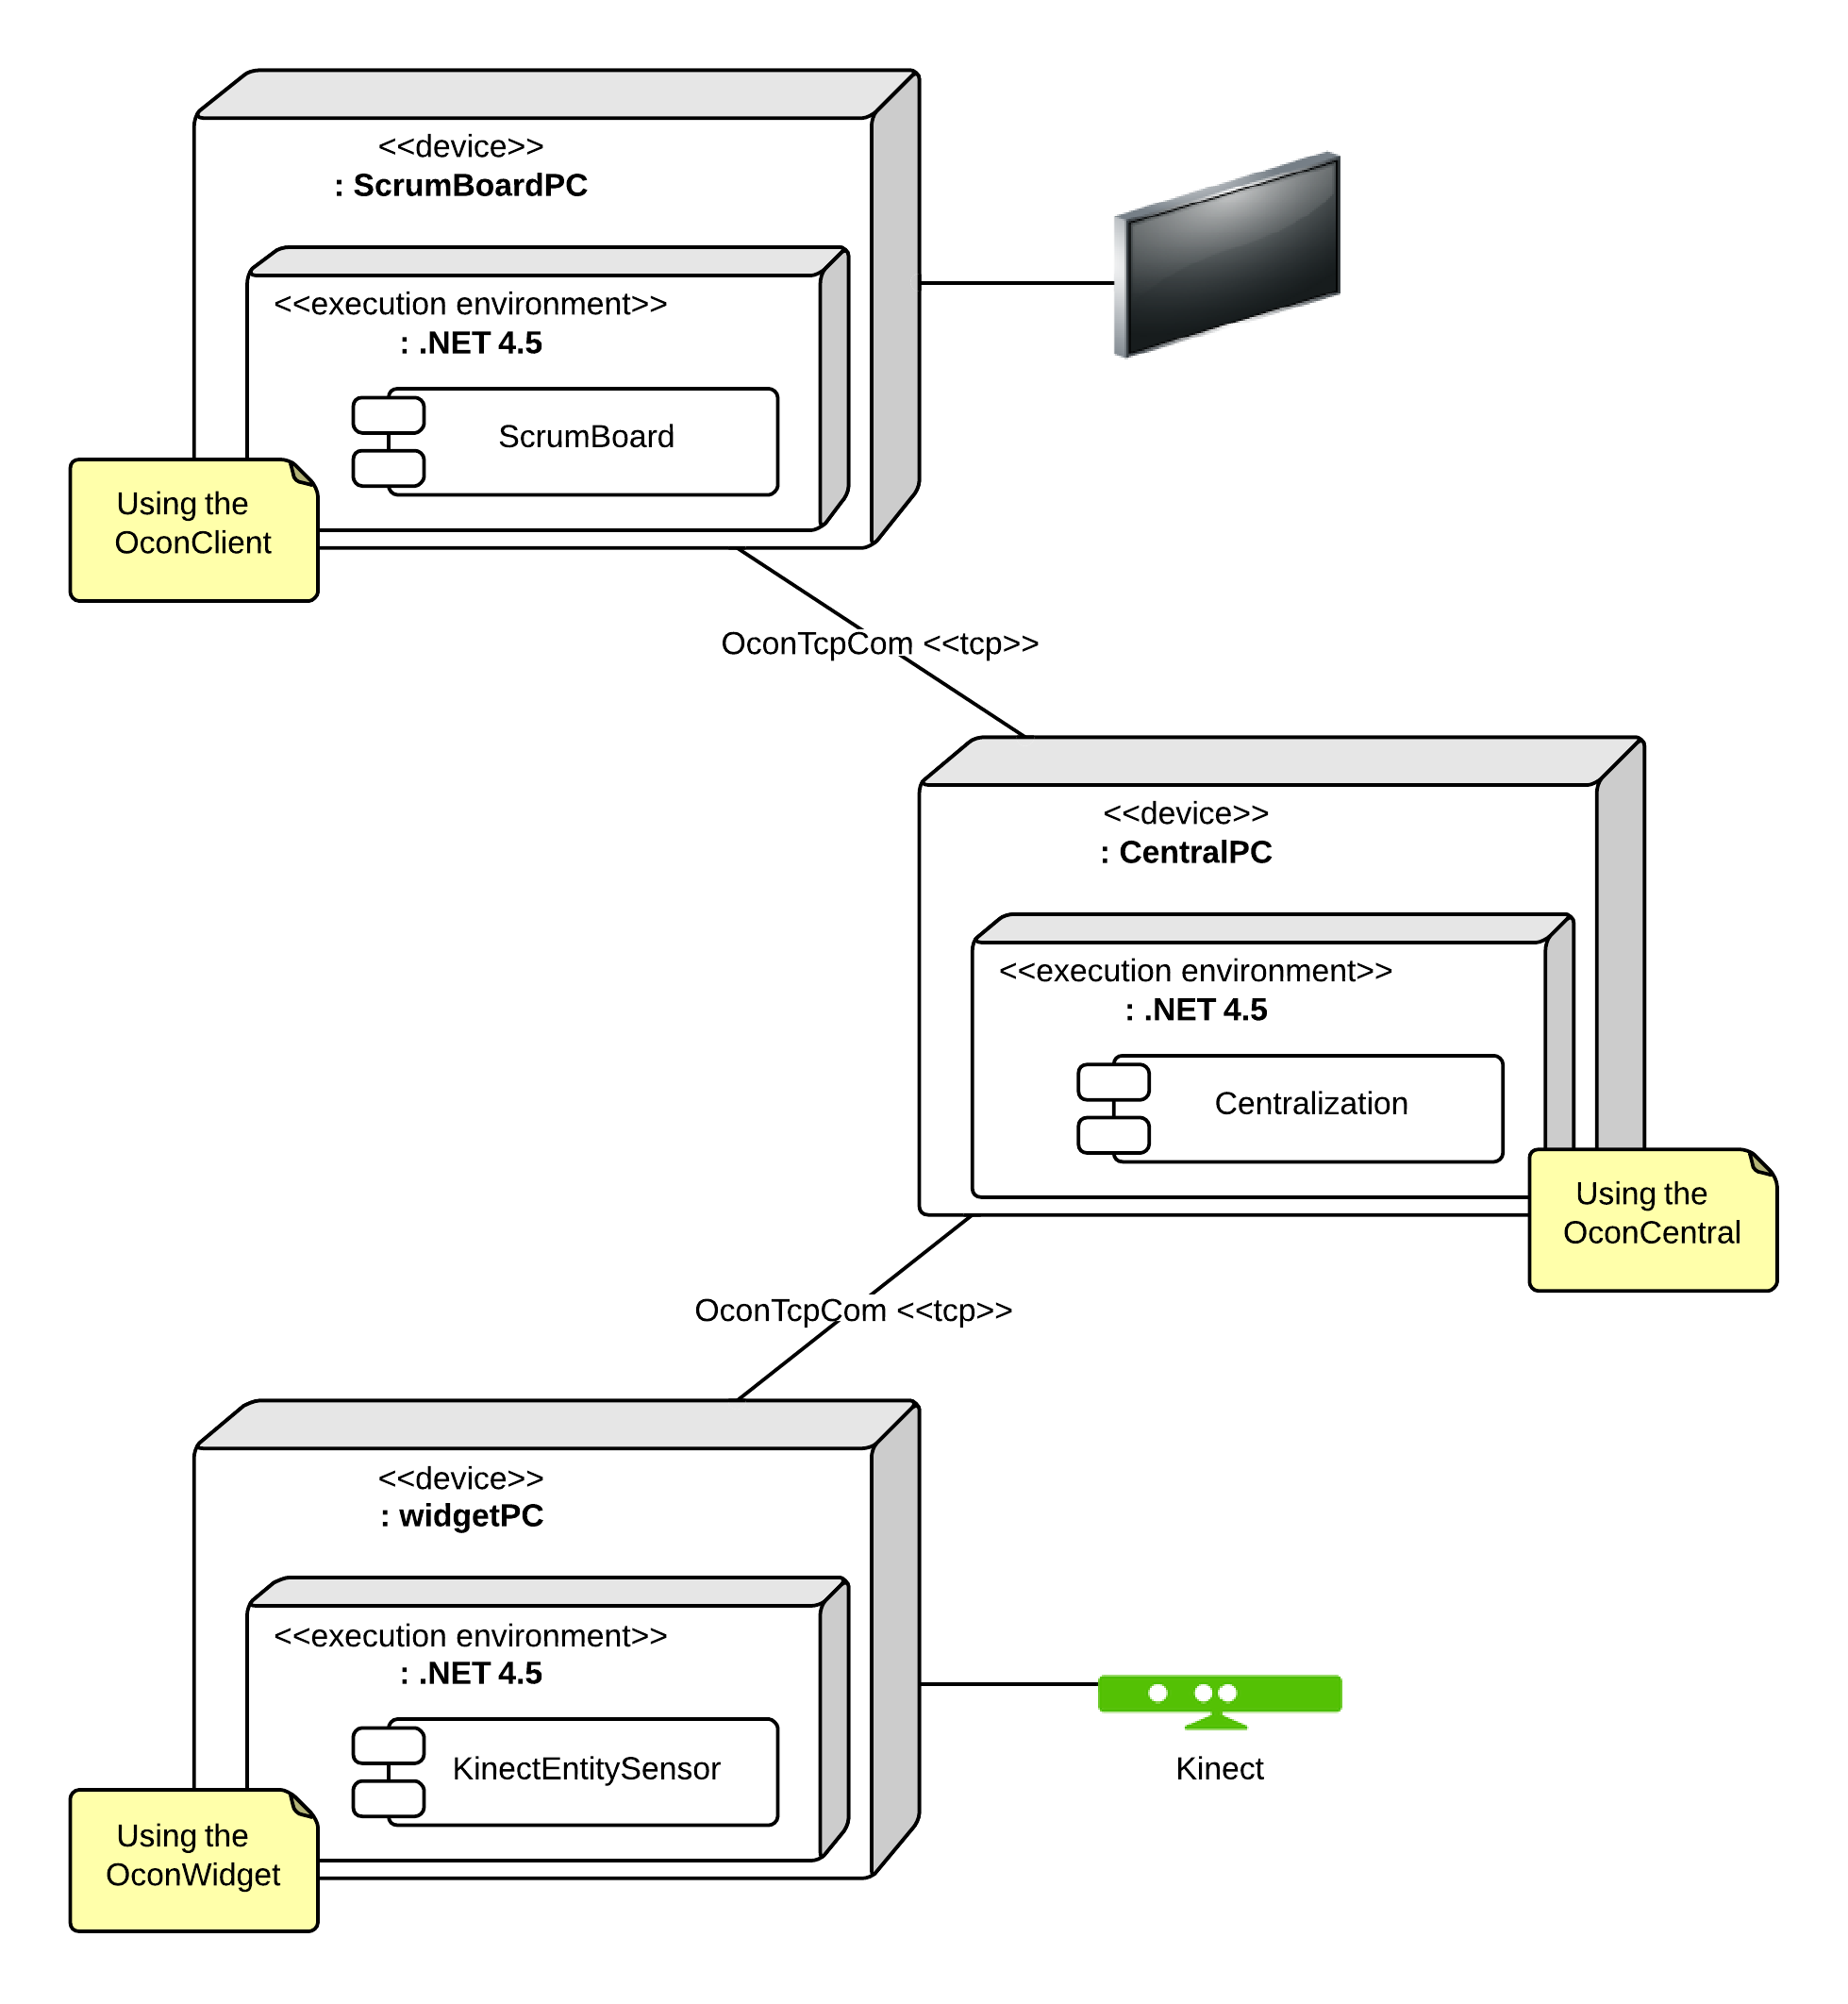
\includegraphics[scale=0.155]{./ProofOfConceptDeployment.png}
\caption{Proof of concept deployment}
\end{center}
\label{fig:ProofofConceptDeployment}
\end{figure}



\subsection{The KinectEntitySensor}
The KinectEntitySensor's task is to gather Context Information and send it to the centralization. This part of the Context-aware Scrumboard implementation involves transferring information to the OconCentral, and it is for that purpose the OconWidget has been implemented. On figure \ref{code:OconWidget} is a snippet of the implementation.
\begin{figure}[H]
\begin{lstlisting}
//Instantiate a logging instance
var log = Console.Out;
//for file logging: new StreamWriter("/file/path/here");

//Instantiate an IOconCom implementation
var com = new OconTcpCom(log);

//Instantiate widget
var widget = new OconWidget(com, log);

//Pass an entity to be added/updated at the central
var entity = new Person() { Name = "Mat", Present = true };
widget.Notify(entity);
\end{lstlisting}
\caption{Widget usage from TestWidget.Program}
\label{code:OconWidget}
\end{figure}

This code is mostly object instantiation followed by passing a hardcoded Person implementation to the OconWidget. Generally the job of this component is to transform captured context information into IEntity implementations and passing them to the OconWidget to be transfered to the OconCentral.



\newpage


\subsection{The centralization}


The centralization has multiple tasks. First of all it's task is to receive Person objects from the KinectEntitySensor and coordinate them accordingly. Second of all it's task is to check registered situation predicates when entities are added or changed. And finally it's task is to notify subscribers when situation predicate states change.


\begin{figure}[H]
\begin{lstlisting}
//Instantiate a logging instance
var log = Console.Out;

//Instantiate an IOconCom implementation
var tcpCom = new OconTcpCom(log);

//Instantiate the context filter
var oconFilter = new OconContextFilter(log);

//Instantiate situations with names and predicates
var closeupSituation = new Situation("Closeup", e => e.OfType<Person>().Count(p => p.Present) == 1);
var standupSituation = new Situation("Standup", e => e.OfType<Person>().Count(p => p.Present) <= 2);

//Add the situations to the filter
oconFilter.AddSituation(closeupSituation, standupSituation);

//Instantiate the central
var central = new OconCentral(oconFilter, tcpCom, log);
\end{lstlisting}
\caption{Central usage from TestCentral.Program}
\label{code:OconCentral}
\end{figure}


\newpage

\subsection{The Scrumboard}

The Scrumboard's task is to firstly register to situations on the Centralization and secondly bind and action with the OconClient which is fired when a subscribed situation's state has changed.

\begin{figure}[H]
\begin{lstlisting}
//Choose a logging instance if any
var log = Console.Out;

//Instantiate a network helper. Here passing the logging target
//alternatively instantiate as new TcpHelper(); if no logging is needed
var comHelper = new OconTcpCom(log);

//Instantiate the client with communication, log, and params of situation names strings
var oconClient = new OconClient(comHelper, log, StandupSituationString, CloseupSituationString);

//Subscribe a delegate to be run when a situation change event is fired
oconClient.SituationStateChangedEvent += (sender, args) => UpdatePicture(args.SituationName, args.State);
\end{lstlisting}
\caption{Client usage from OconScrumBoard.MainViewModel}
\label{code:OconClient}
\end{figure}









\end{document}